Looking back at figure (\ref{intro:production-system}), we realise that we have only been focusing on one part of the global schema. Indeed, we have only dealt with inventory management so far. This part of the course will now focus on what is called "Bill of materials" in which we look at how we can manage the relations between raw materials and final product production.

\section{Model representation and explosion of bill of materials}

The Bill of materials uses a standard representation in terms of graph. The nodes are a set of products : raw materials, final products or temporary products. Temporary products are products which are used to make either other temporary products or final products from either other temporary products or raw materials. The arcs of the graph represents transformations. In figure (\ref{without_st:representation}), the first case where a node $i$ is linked to a node $j$ represents the fact that, somehow, product $i$ is transformed into product $j$, for instance, if we paint a piece of wood (product $i$) it becomes a painted piece of wood (product $j$), or again, if we cut a large piece of iron (product $i$) we transforme it into \emph{several} smaller pieces of iron. The number $n_{ij}$ valuating the arc tells us how many product $i$ we need to produce a single product $j$. If we consider the painting operation, then $n_{ij}=1$, whereas if we consider cutting an iron piece, $n_{ij}\ge 2$ (depending on the situations). The second case represents the fact of assembling products $i$ and $j$ in order to make product $k$. Again, $n_{ik}$ represents the number of product $i$ needed to make one product $k$.

\begin{figure}[h!]
    \centering
    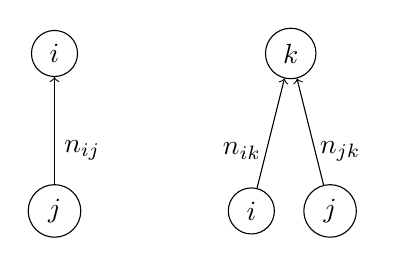
\begin{tikzpicture}
        % first case
        \node[draw, circle] at (0,0) (i) {$i$};
        \node[draw, circle] at (0,-2) (j) {$j$};
        \draw[<-] (i) -- node [below right] {$n_{ij}$} (j);

        % second case
        \node[draw, circle] at (3, 0) (k) {$k$};
        \node[draw, circle] at (2.5, -2) (i2) {$i$};
        \node[draw, circle] at (3.5, -2) (j2) {$j$};
        \draw[->] (i2) -- node[below left] {$n_{ik}$} (k);
        \draw[->] (j2) -- node[below right] {$n_{jk}$} (k);
    \end{tikzpicture}
    \caption{\label{without_st:representation}Bill of materials representation in terms of graph}
\end{figure}

Let's now consider figure (\ref{without_st:first_example}) which shows you a first example of bill of materials and let's extend the notation $n_{ij}$ to any nodes $i$ and $j$ as long as there exists a path from $i$ to $j$ in the graph. Then, $n_{2f}$ represents the number product $2$ needed to produce $1$ final product $f$. How can we compute that value ? It is rather simple : we need $3$ units of product $1$ to produce $1$ unit of product $f$, but we need $2$ unit of product $2$ to produce $1$ unit of product $1$ ; the quantity $n_{2f}$ is then given by $n_{21}\times n_{1f} = 2 \times 3 = 6$, we need $6$ units of procut $2$ to produce $1$ unit of product $f$. In general, the following formula holds : \[ n_{kf} = \prod_{ (i,j)\in Path(k\rightarrow f) } n_{ij} \]

\begin{figure}[h!]
    \centering
    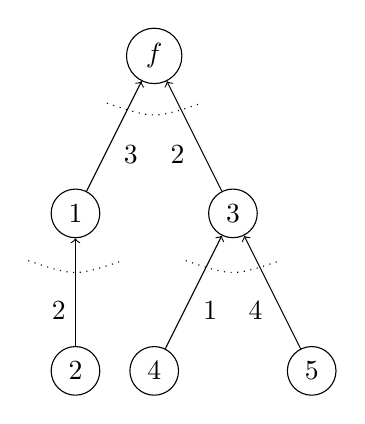
\begin{tikzpicture}
        \draw (0,0) node [draw, circle] (f) {$f$};
        \draw (-1,-2) node [draw, circle] (1) {$1$};
        \draw (-1,-4) node [draw, circle] (2) {$2$};
        \draw (1,-2) node [draw, circle] (3) {$3$};
        \draw (0,-4) node [draw, circle] (4) {$4$};
        \draw (2,-4) node [draw, circle] (5) {$5$};

        \draw[->] (1) -- node (1f) [below right] {3} (f);
        \draw[->] (2) -- node [below left] {2} (1);
        \draw[->] (3) -- node (2f) [below left] {2} (f);
        \draw[->] (4) -- node [below right] {1} (3);
        \draw[->] (5) -- node [below left] {4} (3);

        \draw[dotted] (-.6, -.6) .. controls (0, -.8) .. (.6, -.6);
        \draw[dotted] (-1.6, -2.6) .. controls (-1, -2.8) .. (-.4, -2.6);
        \draw[dotted] (.4, -2.6) .. controls (1, -2.8) .. (1.6, -2.6);
    \end{tikzpicture}
    \caption{\label{without_st:first_example}First example of Bill of Materials}
\end{figure}

It is clear now that if we want to produce a certain number of product $f$ denoted $X_f$, we need to produce at least $X_fn_{if}$ product $i$ so that $X_i\ge X_fn_{if}$. In the following discussion, we will always choose $X_i = X_fn_{if}$ which corresponds to the "conservation of flow" in our system (even though it is not a necessary condition). An other assumption we will make in this chapter, as well as in chapter 2, is that every machine can produce only one kind of product. We will then denote by $i$ both the product and the machine producing it. 

Considering machine $i$, let $\mu_i$ be the maximum speed for producing one product, expressed as items/unit of time, and we define $u_i$ as the "utilization of the resource $i$" which equals : \[ u_i = \frac{X_fn_{if}}{\mu_i}\le 1, \forall i \] Using that definition, it holds that \[ X_f\le\frac{\mu_i}{n_{if}}, \forall i\Leftrightarrow X_f\le\min_i\left( \frac{\mu_i}{n_{if}} \right) \overset{\Delta}{=} X_f^{max} \] where $X_f^{max}$ is the maximum rate at which we can produce product $f$ with respect to the machines we use to produce it. The bottleneck machine(s) can be computed as $\textrm{argmin}_i\left( \frac{\mu_i}{n_{if}} \right)$. This (or these) machine(s) is (are) the one(s) which prevents us from producing more, at a higher rate. 

\section{Production time}

Given a machine $i$, we can compute the operation time needed to produce one item of product $i$ which is simple \[ T_{oi} = \frac{1}{\mu_i} \] We then enhance figure (\ref{without_st:first_example}) with those operation times as a valuation of the arcs. Figure (\ref{without_st:with_toi}) shows such a representation. The operation time has been added as the second element of a couple. The first element will be dealt with in chapter two of this section. The maximum rate $X_f^{max}$ at which we can produce our final product is then given by \[ X_f^{max} = \min_i\left( \frac{1}{T_{oi}n_{if}} \right) \]

\begin{figure}[h!]
    \centering
    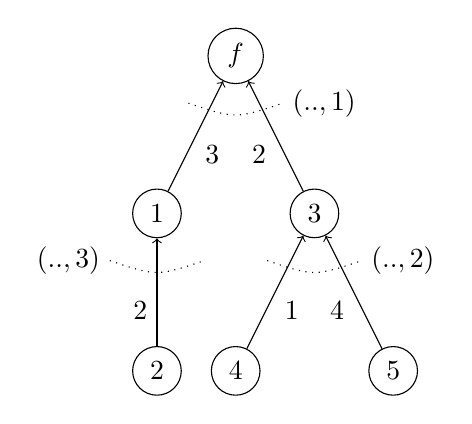
\begin{tikzpicture}
        \draw (0,0) node [draw, circle] (f) {$f$};
        \draw (-1,-2) node [draw, circle] (1) {$1$};
        \draw (-1,-4) node [draw, circle] (2) {$2$};
        \draw (1,-2) node [draw, circle] (3) {$3$};
        \draw (0,-4) node [draw, circle] (4) {$4$};
        \draw (2,-4) node [draw, circle] (5) {$5$};

        \draw[->] (1) -- node (1f) [below right] {3} (f);
        \draw[->] (2) -- node [below left] {2} (1);
        \draw[->] (3) -- node (2f) [below left] {2} (f);
        \draw[->] (4) -- node [below right] {1} (3);
        \draw[->] (5) -- node [below left] {4} (3);

        \draw[dotted] (-.6, -.6) .. controls (0, -.8) .. (.6, -.6) node[right] {$(.., 1)$};
        \draw[dotted] (-1.6, -2.6) node[left] {$(.., 3)$} .. controls (-1, -2.8) .. (-.4, -2.6);
        \draw[dotted] (.4, -2.6) .. controls (1, -2.8) .. (1.6, -2.6) node[right] {$(.., 2)$};
    \end{tikzpicture}
    \caption{\label{without_st:first_example}First example of Bill of Materials}
\end{figure}

Let's start by computing the $n_{if}$ quantities for all $i$, we get :
\[
    \begin{aligned}[l]
        n_{1f} &= 3 & n_{3f} &= 2 & n_{5f} &= 4\times 2 = 8\\
        n_{2f} &= 2\times 3 = 6 & n_{4f} &= 1\times 2 = 2\\
    \end{aligned}
\]
then we can find $X_f^{max}$ as well as the bottleneck machine by doing the following
\[
    \begin{split}
        X_f^{max} &= \min_i\left( \frac{1}{T_{oi}n_{if}} \right)\\
                  &= \min\left( \frac{1}{1\times 3} , \frac{1}{3\times 6} , \frac{1}{1\times 2} , \frac{1}{2\times 2} , \frac{1}{2\times 4} \right)\\
                  &= \min\left( \frac{1}{3} , \frac{1}{18} , \frac{1}{2} , \frac{1}{4} , \frac{1}{8} \right)\\
                  &= \frac{1}{18}\\
                  \\
        bottleneck &= \textrm{arg}\min_i\left( \frac{1}{T_{oi}n_{if}} \right) = 2\\
    \end{split}
\]
Note that, in this case, the bottleneck machine is the one with the highest operation time. This is NOT a general rule, and it's easy to find a counter example : consider a final product $f$ which is made by assembling a hundred small pieces with one big one. Clearly, even if the machine which produces the small pieces is efficient, it is \emph{possible} that making a hundred of these pieces may be longer than producing one other piece, even bigger. But again, this isn't always the case. The only way to solve for the bottleneck machine problem is to look at both the operation time and the number of products required to produce the final product. 

\section{Batch production}

A batch $b_i$ can be defined as the number of items $i$ the machine produces without interuption before releasing it to ther machines. Let's suppose that we want to produce a batch of final product $b_f$, how much time do we need to do it ? In this section, we will try to answer that question considering that our batch sizes are $b_i = b_fn_{if}$, which is not necessary, but simpler. In general however, you often have external constraints (linked to the technology you use for example) which imposes a minimum batch size or a maximum batch size, so that : 
\[ b_i^{min} \le b_i \le b_i^{max}, \forall i \]
From that constraint, we can deduce the following
\[
    \begin{split}
        \Rightarrow & b_i^{min} \le b_fn_{if} \le b_i^{max}, \forall i \\
        \Rightarrow & \frac{b_i^{min}}{n_{if}} \le b_i \le \frac{b_i^{max}}{n_{if}}, \forall i\\
        \Rightarrow & \max_i\left( \frac{b_i^{min}}{n_{if}} \right) \le b_f \le \min_i\left( \frac{b_i^{max}}{n_{if}} \right)
    \end{split}
\]
Since the batch size $b_f$ has to be an integer, we have to make sure that this interval contains at least on integer value, otherwise, we cannot use $b_i = b_fn_{if}$ as a batch size. 

Considering that relation to hold however, we can compute the production time for a given batch as \[ T_{i,prod}(b_i) = T_{oi}b_i = T_{oi}b_fn_{if} \] which now allows us to compute the time takes to go from one raw material (a leaf of the tree in our graph representation) to the final product (root of tree). Considering $\mathcal P_k$ as the path going from the raw material $k$ to the final product in our graph, it holds that \[ T_{\mathcal P_k} = \sum_{j\in\mathcal P_k}T_{j,prod}(b_j) = b_f\sum_{j\in\mathcal P_k} T_{oj}n_{jf} \] This relation tells us about how much time we would need to produce a batch of final product $b_f$ since \[ T_{prod}(b_f) = \max_{\mathcal P_k}\left( T_{\mathcal P_k}(b_f) \right) \]

Up to now, we have considered choosing a batch size $b_f$ and compute the time needed to produce it. But we can as well use the established formulas in the other way to compute the maximum batch size allowed in order respect a certain constraint on production time. For instance, let's say we want to respect the condition $T_{prod}(b_f) \le T^{max}$ meaning that we do not want to produce more than $T^{max}$ units of time. Then it still holds that 
\[
    \begin{split}
        T_{prod}(b_f) \le T^{max}
            &\Leftrightarrow b_f\max_{\mathcal P_k}\left( b_f\sum_{j\in\mathcal P_k} T_{oj}n_{jk} \right) \le T^{max}\\
            &\Leftrightarrow b_f \le \frac{T^{max}}{ \max_{\mathcal P_k}\left( \sum_{j\in\mathcal P_k} T_{oj}n_{jk} \right) }
    \end{split}
\] which tells us about the maxumum size we can use for a batch in order to fullfill that constraint. 

One final consideration is to be taken regarding the rotation of batches. Let's say we want to produce $X_f^* \le X_f^{max}$ final products. We introduce the variable $D$ as the difference in time between the moment a batch is produced and the moment a subsequent batch is produced so that \[ X_f^* = \frac{b_f}{D} \] (number of items of the final product over the time of a "period" of production) The figure (\ref{without_st:cycle}) illustrates this notion.

\begin{figure}[h!]
    \centering
    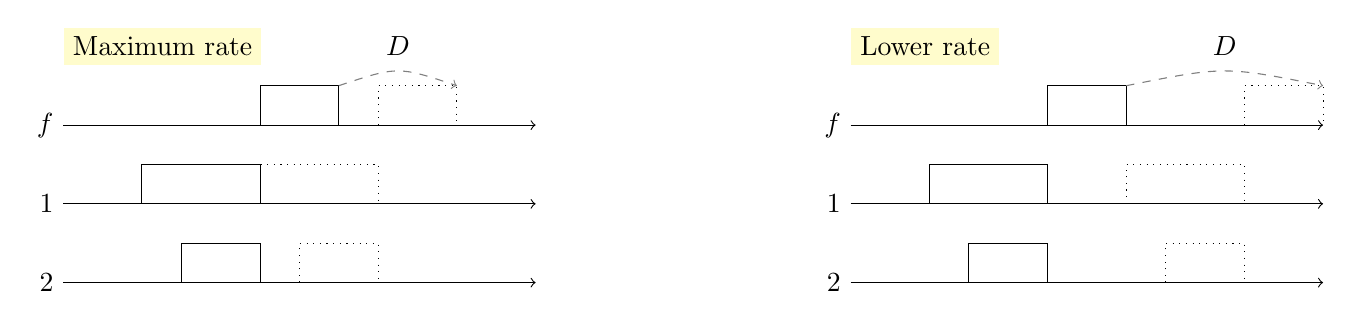
\begin{tikzpicture}

    % maximum rate
    \draw (0, 1) node [right, fill=yellow!20] {Maximum rate};

    \draw[->] (0,0) node[left] {$f$} -- (6,0);
    \draw (2.5, 0) rectangle (3.5, .5);
    \draw[dotted] (4, 0) rectangle (5, .5);

    \draw[->] (0,-1) node[left] {$1$} -- (6,-1);
    \draw (1, -1) rectangle (2.5, -.5);
    \draw[dotted] (2.5, -1) rectangle (4, -.5);

    \draw[->] (0,-2) node[left] {$2$} -- (6,-2);
    \draw (1.5, -2) rectangle (2.5, -1.5);
    \draw[dotted] (3, -2) rectangle (4, -1.5);

    \draw[->, dashed, gray] (3.5, .5) .. controls (4.25, .75) .. (5, .5);
    \draw (4.25, 1) node {$D$};
    
    % lower rate
    \draw (10, 1) node [right, fill=yellow!20] {Lower rate};
    \draw[->] (10,0) node[left] {$f$} -- (16,0);
    \draw (12.5, 0) rectangle (13.5, .5);
    \draw[dotted] (15, 0) rectangle (16, .5);

    \draw[->] (10,-1) node[left] {$1$} -- (16,-1);
    \draw (11, -1) rectangle (12.5, -.5);
    \draw[dotted] (13.5, -1) rectangle (15, -.5);

    \draw[->] (10,-2) node[left] {$2$} -- (16,-2);
    \draw (11.5, -2) rectangle (12.5, -1.5);
    \draw[dotted] (14, -2) rectangle (15, -1.5);

    \draw[->, dashed, gray] (13.5, .5) .. controls (14.75, .75) .. (16, .5);
    \draw (14.75, 1) node {$D$};

    \end{tikzpicture}
    \caption{\label{without_st:cycle}GANT diagram with production cycle}
\end{figure}